\documentclass{article}
\title{ECE 311 -- Homework 5}
\usepackage[margin=1in]{geometry}
\usepackage{graphicx}
\usepackage{pdfpages}
\usepackage{fancyhdr}
\usepackage{enumitem}
\usepackage{pdfpages}
\usepackage{amsmath}
\usepackage{amssymb}
\usepackage{float}
\pagestyle{fancy}
\fancyhf{}
\fancyhead[L]{Gianni Avilan-Losee}
\fancyhead[C]{ECE 311}
\fancyhead[R]{Homework 5}
\fancyfoot[C]{\thepage}
\usepackage{microtype}
\usepackage{textcomp, gensymb}
\author{Gianni Avilan-Losee}
\setcounter{section}{1}
\begin{document}
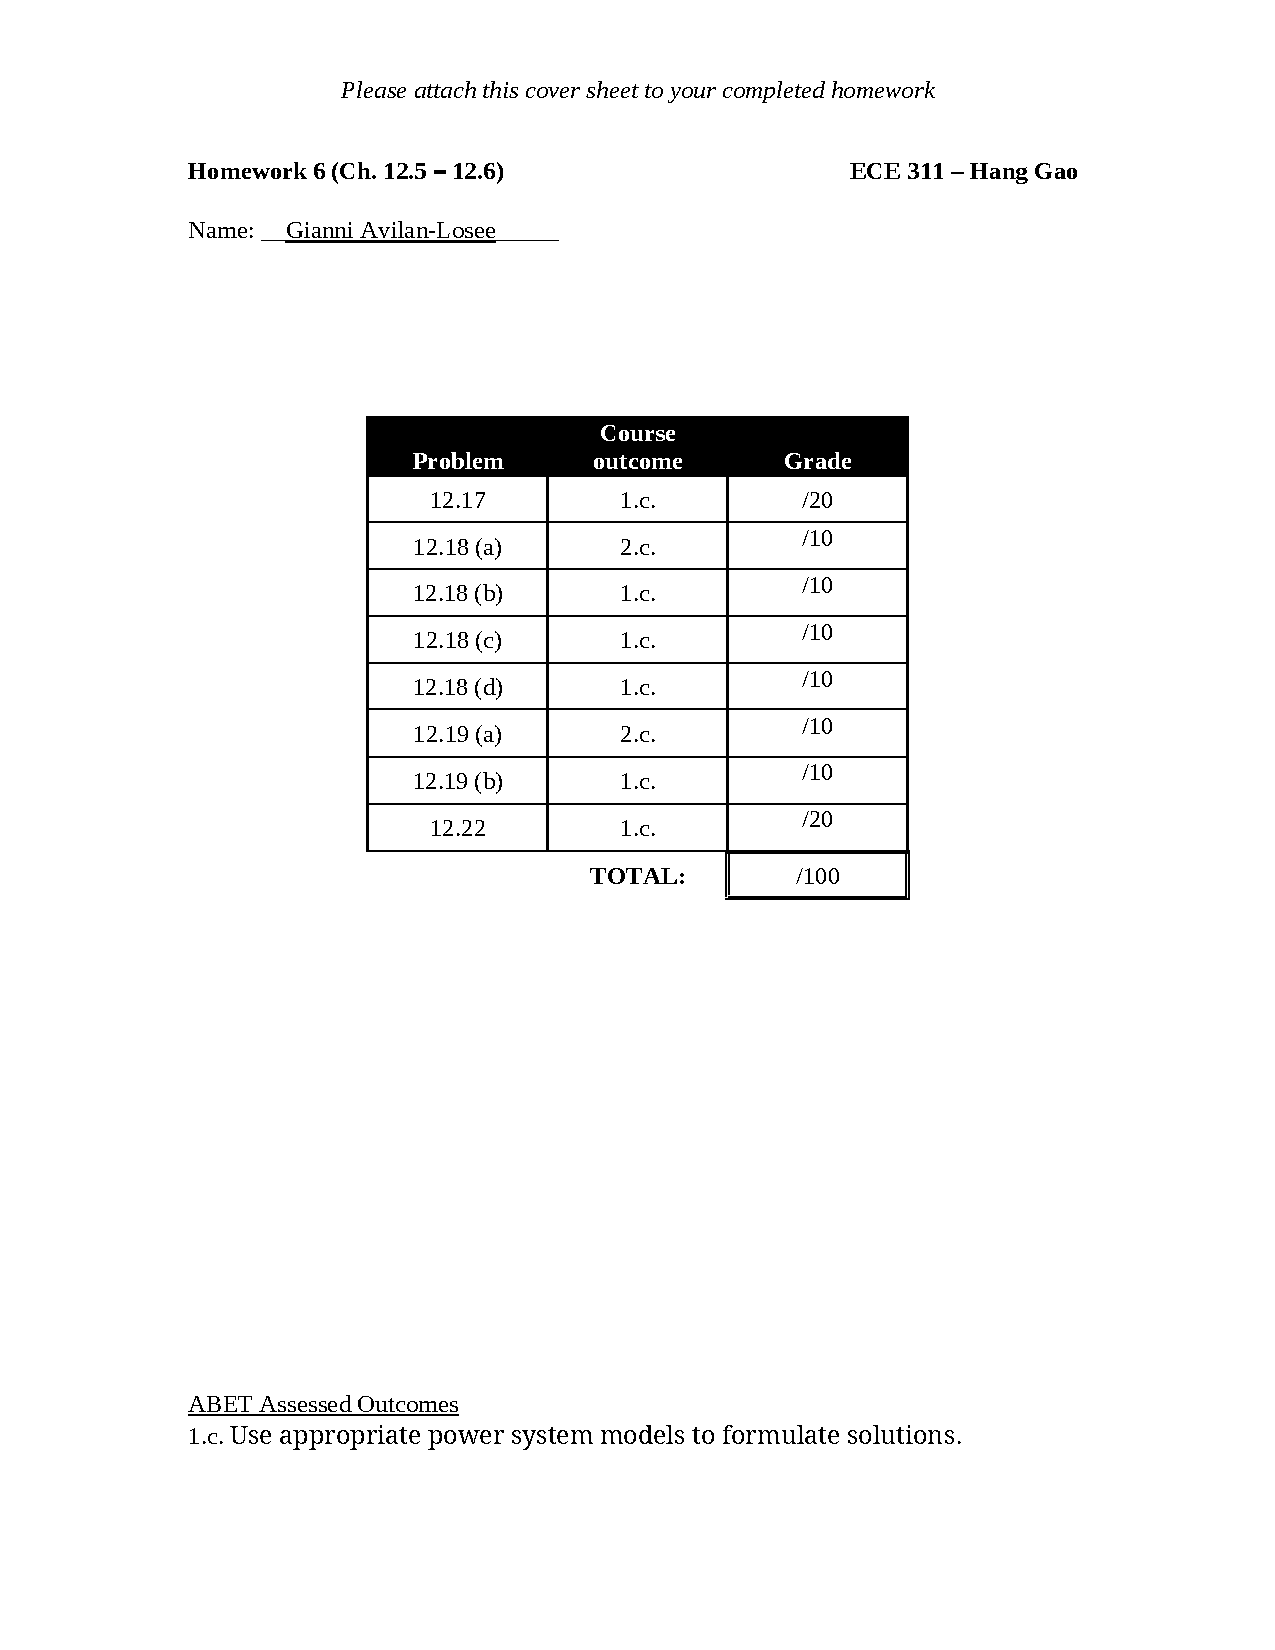
\includepdf[pages=-]{homework-6_cover-page.pdf}
\begin{enumerate}[label=\thesubsection]
	\setcounter{section}{12}
	\setcounter{subsection}{17}
	\item Using the power angle equation for reactive power
		\[
			Q = 3 \frac{V_o}{X_s} (E_f\cos{\delta} - V_o),
		\]
		and assuming that \(\delta = 90\degree\), since the generator is operating at its maximum power, solve for the reactive power \(Q\) as
		\[
			Q = 3 \frac{277.13}{5}(-277.13) = -46.081^{\mathrm{kVAR}}.
		\]
		\setcounter{subsection}{18}
		\item
			\begin{enumerate}[label=\alph*)]
				\item Terminal voltage may be found as a function of the transmission line current, which itself is a function of the power angle \(\delta\). Finding power angle \(\delta\) and effective field voltage \(E_f\) as a function of \(P\) and \(Q\),
					\begin{align*}
						&P = 1 \times 10^9 = \frac{3 V_o E_f}{X} \sin{\delta} \to E_f \sin{(\delta)} = \frac{PX}{3 V_o} = 62.984^{\mathrm{kV}} \\
						&Q = 0 = \frac{3V_o}{X_s}(E_f \cos{(\delta)} - V_o) \to E_f \cos{(\delta)} = V_o = 63.51^{\mathrm{kV}}.
					\end{align*}
					Therefore, 
					\[
						\overline{E}_f = E_f\cos{(\delta)} + jE_f\sin{(\delta)} = 63.51 + j62.98^{\mathrm{kV}},
					\]
					and
					\[
					  \delta = 44.76\degree.
					\]
					Then, we may find current as 
					\[
						\overline{I}_a = \frac{\overline{E}_f - \overline{V}_o}{\overline{X}} = \frac{89.44 \angle{44.76\degree} - 63.51\angle{0\degree}}{12 \angle{90\degree}} =  5.25 \angle{0 \degree}^{\ \mathrm{kA}}.
					\]
					Then, finding line voltage,
					\[
						\overline{V}_l = \overline{V}_o + \overline{I}_a \overline{X}_l = \frac{110}{\sqrt{3}}\angle{0\degree} + ([5.25 \angle{0\degree}] \times [3\angle{90\degree}]) = 65.43 \angle{13.93\degree}^{\ \mathrm{kV}}.
					\]
					Finally, line-to-line terminal voltage may be found as 
					\[
						65.43 \times \sqrt{3} = 113.33^{\mathrm{kV}}.
					\]
				\item Equivalent field voltage, as shown in the previous step, is
					\[
						E_f = |\overline{E}_f| = 89.44^{\mathrm{kV}}.
					\]
				\item Real power output at the generator terminals is \(P\), that is,
					\[
						P_t = P = 1^{\mathrm{GW}}.
					\]
				\item Reactive power output at the terminals may be found using \(\alpha\), the angle between terminal voltage and \(E_f\), as
					\[
						Q_t = \frac{3V_t}{X_s}(E_f \cos{(\alpha)} - V_t) = \frac{3(65.43)}{9}(89.44\cos{(30.83\degree)} - 65.43) = 248^{\mathrm{MVAr}}.
					\]
			\end{enumerate}
			\setcounter{subsection}{19}
			\item
				\begin{enumerate}[label=\alph*)]
					\item Pullover power occurs when \(\delta = 90\degree\), and so 
						\[
							P_{\mathrm{max}} = \frac{3V_oE_f}{X_s} = \frac{3 \times \frac{15}{\sqrt{3}} \times 14}{5} = 72.75^{\mathrm{MW}}.
						\]
					\item To increase \(P_{\mathrm{max}}\) to \(87.3^{\mathrm{MW}}\) using a higher excitation voltage, solving for \(E_f\), 
						\[
							E_f = \frac{P_{\mathrm{max}}X_s}{3V_o} = \frac{87.3 \times 5}{3 \times \frac{15}{\sqrt{3}}} = 16.8^{\mathrm{kV}}.
						\]
		    \end{enumerate}
				\setcounter{subsection}{22}
			\item Reactive power consumed by a motor is given by
				\[
					Q = \frac{V_t}{X_s}(V_t - E_f\cos{(\delta)}), 
				\]
				and so, using \(Q = -3^{\mathrm{MVAr}}\) and \(\delta = 0\degree\),
				\[
					E_f = -\frac{Q X_s}{V_t} + V_t = \frac{3 \times 5}{5} + 5 = 8^{\mathrm{kV}}.
				\]
\end{enumerate}
\end{document}
